%%%%%%%%%%%%%%%%%%%%%%%%%%%%%%%%%%%%%%%%%%%%%%%%%%%%%%%%%%%%%%%%%%%%%%
% How to use writeLaTeX: 
%
% You edit the source code here on the left, and the preview on the
% right shows you the result within a few seconds.
%
% Bookmark this page and share the URL with your co-authors. They can
% edit at the same time!
%
% You can upload figures, bibliographies, custom classes and
% styles using the files menu.
%
% If you're new to LaTeX, the wikibook is a great place to start:
% http://en.wikibooks.org/wiki/LaTeX
%
%%%%%%%%%%%%%%%%%%%%%%%%%%%%%%%%%%%%%%%%%%%%%%%%%%%%%%%%%%%%%%%%%%%%%%
\documentclass{tufte-handout}

%\geometry{showframe}% for debugging purposes -- displays the margins

\usepackage{amsmath}

% Set up the images/graphics package
\usepackage{graphicx}
\setkeys{Gin}{width=\linewidth,totalheight=\textheight,keepaspectratio}
\graphicspath{{graphics/}}

\title[How to start with GitHub and git for R?]{How to start with GitHub and git for \textnormal{\textsf{R}}?}
\author[Szymon M. Drobniak]{Szymek Drobniak}
% \date{}  % if the \date{} command is left out, the current date will be used

% The following package makes prettier tables.  We're all about the bling!
\usepackage{booktabs}

% The units package provides nice, non-stacked fractions and better spacing
% for units.
\usepackage{units}

% The fancyvrb package lets us customize the formatting of verbatim
% environments.  We use a slightly smaller font.
\usepackage{fancyvrb}
\fvset{fontsize=\normalsize}

% Small sections of multiple columns
\usepackage{multicol}

% Provides paragraphs of dummy text
\usepackage{lipsum}

% These commands are used to pretty-print LaTeX commands
\newcommand{\doccmd}[1]{\texttt{\textbackslash#1}}% command name -- adds backslash automatically
\newcommand{\docopt}[1]{\ensuremath{\langle}\textrm{\textit{#1}}\ensuremath{\rangle}}% optional command argument
\newcommand{\docarg}[1]{\textrm{\textit{#1}}}% (required) command argument
\newenvironment{docspec}{\begin{quote}\noindent}{\end{quote}}% command specification environment
\newcommand{\docenv}[1]{\textsf{#1}}% environment name
\newcommand{\docpkg}[1]{\texttt{#1}}% package name
\newcommand{\doccls}[1]{\texttt{#1}}% document class name
\newcommand{\docclsopt}[1]{\texttt{#1}}% document class option name

\begin{document}

\maketitle% this prints the handout title, author, and date

\begin{abstract}
\noindent This documnet describes the basics of using \texttt{git} and \textit{GitHub}\footnote{It is assumed, that the user has the necessary prerequisites in place. These would be: \texttt{git} installed in your OS (often it's present by default, if not - go to \url{https://git-scm.com}); the \textit{GitHub Desktop} app downloaded and installed from \url{https://desktop.github.com/download/}; an account setup on \url{https://github.com}} - one of the most widely used version-control systems. It is not meant to be a complete guide or an exhaustive introduction, but hopefully it will provide an easy-enough start to most fresh users.
\end{abstract}

%\printclassoptions

\section[What is git?]{What is \textnormal{\texttt{git}}?}\label{sec:what-git}

\newthought{Although not the same thing}, \texttt{git} and \textit{GitHub} are related. \texttt{git} is a version-conrol system. It is a small app installed locally, that stores in each of its local repositories the modification history of all repository files. Usually, a repository is a folder where \texttt{git} was initiated\footnote{It can be done using the \texttt{git} program, but it can also be done in a much simpler way using the desktop \textit{GitHub} app - see below.}

Repositories that are kept locally are visible only to you. However, you can synchronise them to a remote, online instance of a repository. in such case, you can both send your changes to the online one (they become integrated in it, with the history of modifications kept) or download changes introduced by others if the repository is shared with multiple contributors. There are several main operations with their characteristic \texttt{git}-lingo names\footnote{Note that I will provide selected, easiest ways to perform some of the \texttt{git} operations;many can be done in several ways, I'll leave exploration of possibilities to you.}:
\begin{itemize}
    \item \textbf{Commit} - which means recording all changes done to the files in a repo as "registered" (i.e., included in the history of modifications of a repo);
    \item \textbf{Push} - which means sending the changes commited in the local repo to its remote, online version - such changes are integrated there if you have writing privileges in the repo, or are queued for review and integration as so-called \textbf{Pull Requests};
    \item \textbf{Pull} - an operation of downloading changes from the online repo, to integrate them into our local copy of the repository\footnote{Pulling and pushing can result in changes to be incorporated silently - if they cause no conflicts or unexpected overwriting. Otherwise, they usually generate an error with recommendations on how to resolve conflicts, or force the changes to go through regardless.};
    \item \textbf{Fork} - if you want to work on a repository but have no permission to modify it, you can fork it to your GitHub \textit{account} - it will become your local copy of the parent repo; in it, you can introduce modifications, you can also synchronise your repo with its parent if needed; any changes you introduce can be pushed back to the original repository, where they will create a pull request, for review by the original repo's owners;
    \item \textbf{Clone} - it means creating your own local copy of some online repository, to which you have access (either as its owner, or contributor).
\end{itemize}

\section{How to start using it?}
\subsection{Your user account}

\newthought{You need to have} a user account\footnote{If you happen to be emplyed by a university or other educational institution - you can apply for a free (!) \textit{GitHub Pro} account. It has to be renewed every two years and it gives you access to many advanced functionalities of the service - among others, you have free access to the Copilot, a \textit{GitHub} AI that can help you write better code, or just find ways of doing things much faster. See  \url{https://github.com/education} for more info.}\footnote{\textit{GitHub} account is free and public - everyone can see it. However, not all your repositories are publically visible - outside of our account, users will be able to see only repositories marked as \textit{Public} by you. \textit{Private} repos are visible only to their owners and people you invite to each of them as contributors.} on \texttt{github.com}. Keep your username in mind as it is an important piece of information you will use linking your local projects with your online account. Exploring the webpage, or your future repos, you will notice, that many things (e.g., adding files, adding readme documents, etc.) can be done through the website. However, I do not recommend this - try to use local \texttt{git} or \textit{GitHub Desktop} to communicate with your online repo (many apps - such as \textit{RStudio} or \textit{VSCode} - also have their own \texttt{git} routines communicating the app and its projects with online \textit{GitHub} instances of each repo.

In order to keep your \textit{GitHub} clean, try to adhere to several simple rules:
\begin{itemize}
    \item always keep each project in a separate folder that then becomes your \texttt{git} repository;
    \item make very deliberate use of \texttt{.gitignore} files - its a file that can reside in your repo's main directory and it contains representations of files and/or folders that should not be tracked for changes and synchronised with your online repo;
    \item always accompany your repo with a readme file explaining what the repo is etc.
\end{itemize}

\subsection{Interacting with online GitHub}

To create a repository online, just click the green \textit{New} button (fig.~\ref{fig:git_repo_online}), name your repository, decide whether it should be private or public, and setup some additional minor details. After creating it, you will be redirected to its website - its URL address is the simplest way to identify a repository.

\begin{marginfigure}
    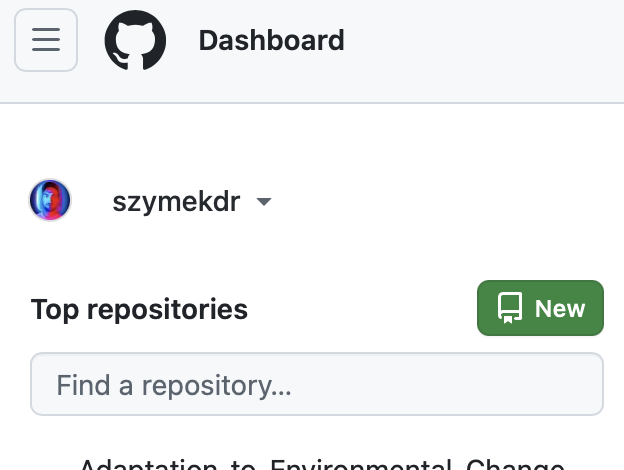
\includegraphics[width=1\linewidth]{Zrzut ekranu 2024-12-20 o 11.57.42.png}
    \caption{Creating a new repo online.}
  \label{fig:git_repo_online}
  % \setfloatalignment{b}
\end{marginfigure}

\subsection{Prerequisites for RStudio and VSCode}

In order to use \texttt{git} in \textit{RStudio} or \textit{VSCode} - you need several additional resources:

\begin{itemize}
    \item RStudio - install the following packages: \texttt{usethis}, \texttt{gitcreds};
    \item VSCode - assuming you want to use it with \textsf{R}: install the above packages through \textsf{R}, and (for a betetr experience) a few VSCode extensions (\texttt{Git Graph}, \texttt{GitHub Copilot}, \texttt{Git History}).
\end{itemize}

\section{Creating a new repository}

\subsection{RStudio}

\texttt{git} will only work, if you are inside of a R Project - make sure to create it in the folder you wish to turn into your new repository\footnote{You can actually create a new R project with a version control environment - check RStudio documentation how to do it.}

Once in an existing project, run the following:

\begin{verbatim}
usethis::use_git()
\end{verbatim}

This function will setup a local repository for the active project, ask you whether you want to commit all files already existing in it (pick \textit{Yes} if you have few small files or in generalk your project is small, otherwise I would first create and edit the \texttt{.gitignore} file to exclude the biggest files from tracking). It may also ask you to restart to display a new panel (\textit{Git}) in the upper right panel of RStudio.

Before you can link your local repo to an online one - you need to set access permissions for RStudio. First, see if any credentials already exist in your RStudio:

\begin{verbatim}
gitcreds::gitcreds_get()
\end{verbatim}

In my case the output looks like this:

\begin{verbatim}
<gitcreds>
  protocol: https
  host    : github.com
  username: PersonalAccessToken
  password: <-- hidden -->
\end{verbatim}

indicating existing credentials. A message about no credentials will be generated if you have never set up \textit{GitHub} before. In such case you will first need to generate a personal access token via \url{github.com}. On your profile page click your avatar, got to \textbf{Settings}, then \textbf{Developer settings}, and then \textbf{Personal access tokens (classic)}. Click \textbf{Generate new token} - there you can pick services you want this token to grant access to (if it's only for you you can tick all). You will be given with a long alfanumeric string (the token) - copy it and (if needed) write it down somwewhere (once you exit the settings page, you will not be able to display it). The copied token can then be used by running the function \texttt{gitcreds::gitcreds\_set()} and providing there the token as your password.

Once your \textit{RStudio} has access to your account, you can run the following code:

\begin{verbatim}
usethis::use_github(private = TRUE)
\end{verbatim}

This will create an online instance of your repo, push all existing committed changes to it, and set it private (you can also set it as public by changing the option \texttt{private} to \texttt{TRUE} - but most likely you will first want to publish your repos privately\footnote{Any private repository can always be made public. The reverse is not possible - public repos must remain public.}).

The \textit{Git} panel will give you access to all basic operations on your repo. You can \textit{Pull} from the remote (download online changes), select and commit any files with local changes (they will appear in the panel), and \textit{Push} any previously committed changes to the online repository.

\begin{figure}
    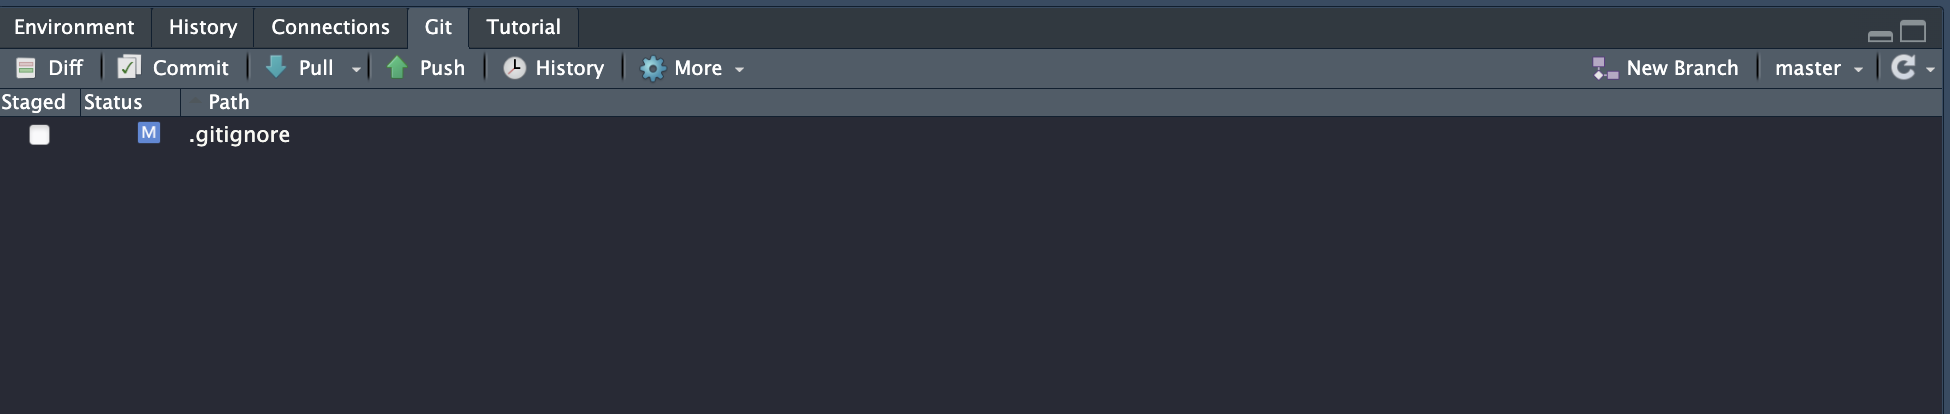
\includegraphics[width=1\linewidth]{Zrzut ekranu 2024-12-20 o 14.07.03.png}
    \caption{The Git panel in RStudio with one changed, uncommitted file.}
    \label{fig:gitpanel}
    \setfloatalignment{t}
\end{figure}

\subsection{VSCode}

If using \textit{VSCode} with \textsf{R} - the way of setting up a \texttt{git} repo in a project folder, and connecting it to an online one works in the same way\footnote{Note, that in \textit{VSCode} you usually don't have to use \texttt{gitcreds} functions to setup access to online \textit{GitHub} - the app is by default connected to \textit{GitHub} (you can log in in \textit{VSCode} to your account directly)}. Pulling and pushing stuff is done via a \textbf{Refresh} button available in the \textbf{Source control} panel (can be accessed in the left bottom corner of the app window; see fig.~\ref{fig:source-control}). The same panel allows you to select files with changes for committing (\textbf{Stage} them), and to actually commit them.

\begin{marginfigure}
    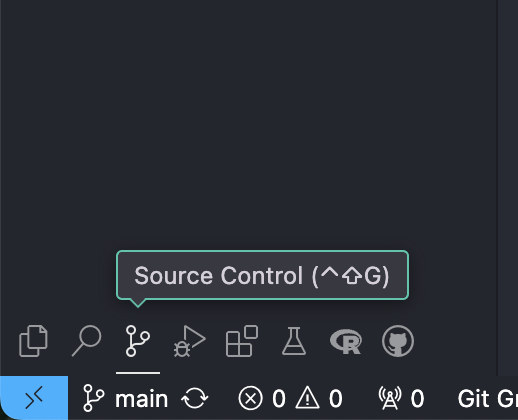
\includegraphics{Zrzut ekranu 2024-12-20 o 14.14.45.png}
    \caption{Location of the Source control panel.}
    \label{fig:source-control}
\end{marginfigure}

\subsection{GitHub Desktop}

I don't recommend creating new repositories in \textit{GitHub Desktop} - doing this via \textit{RStudio} or \textit{VSCode} is much better and ensures they are connected with the correct local folder.

Managing existing repositories in \textit{GitHub Desktop} is very easy. First, you have to add an existing repo by using the \textbf{Add Existing Repository...} option (fig.~\ref{fig:ghd-add}).

\begin{figure}
    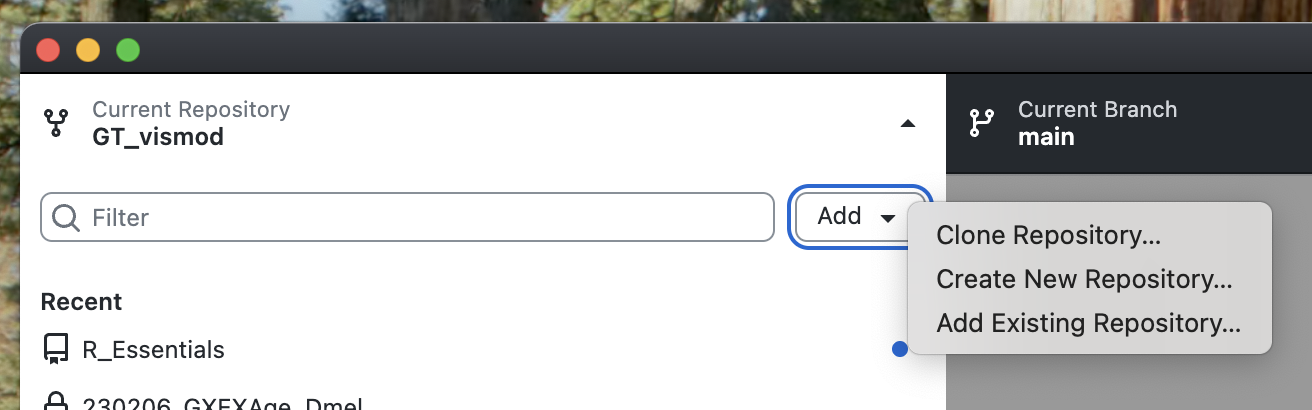
\includegraphics[width=1\linewidth]{Zrzut ekranu 2024-12-20 o 14.23.07.png}
    \caption{How to add an existing repo to GitHub Desktop?}
    \label{fig:ghd-add}
\end{figure}

After adding a repo, it will be available from the \textbf{Current Repository} list later, so you only have to add it once.

For active repo, the program displays files with uncommitted changes (you can actually preview the changes if needed; fig.~\ref{fig:ghd-window}), and at the bottom you can add comments and commit selected files. Once comitted, you can push changes to the remote (fig.~\ref{fig:ghd-push}) or pull things to the local repo (by clicking \textbf{Fetch origin} in the top part of the window.

\begin{figure}
    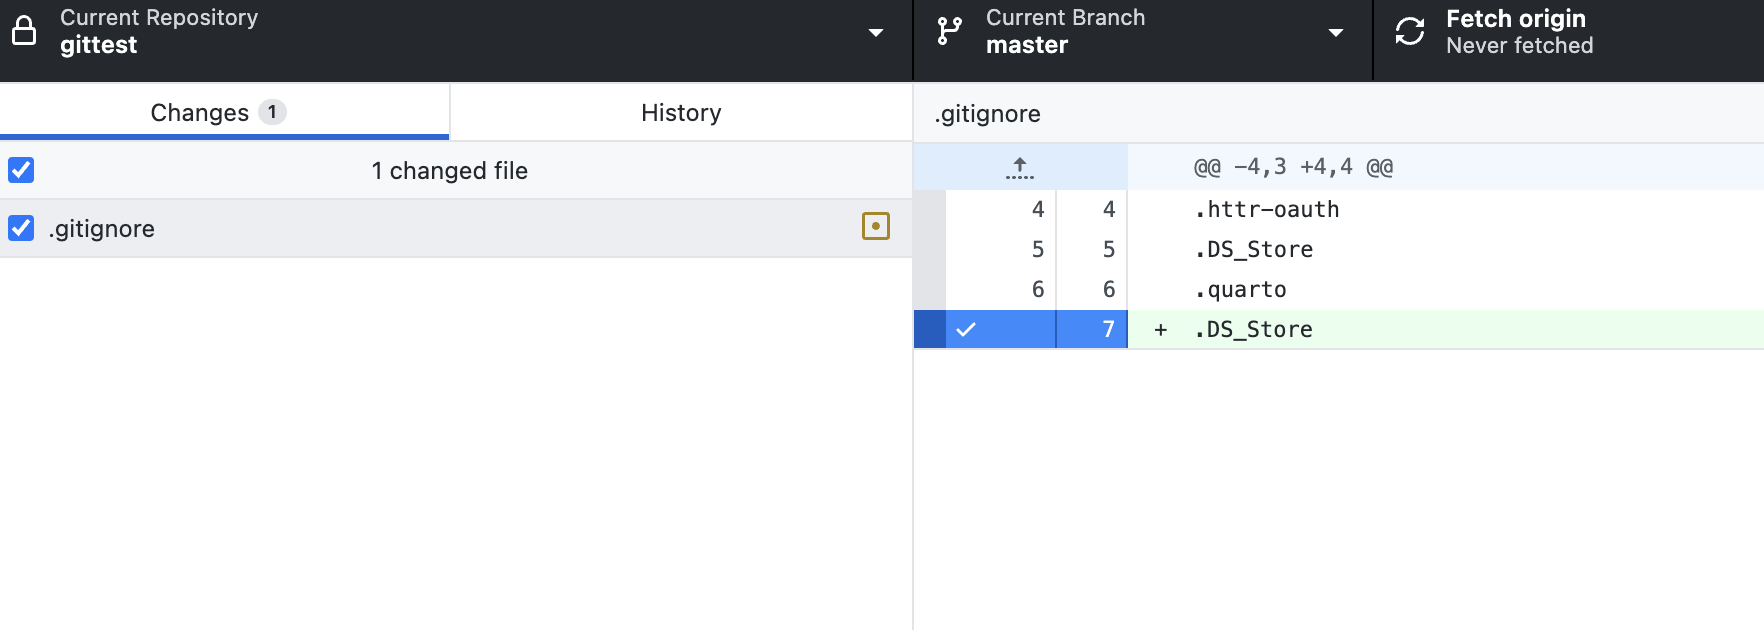
\includegraphics[width=1\linewidth]{Zrzut ekranu 2024-12-20 o 14.27.24.png}
    \caption{GitHub Desktop window with one uncommitted file.}
    \label{fig:ghd-window}
\end{figure}

\begin{figure}
    \centering
    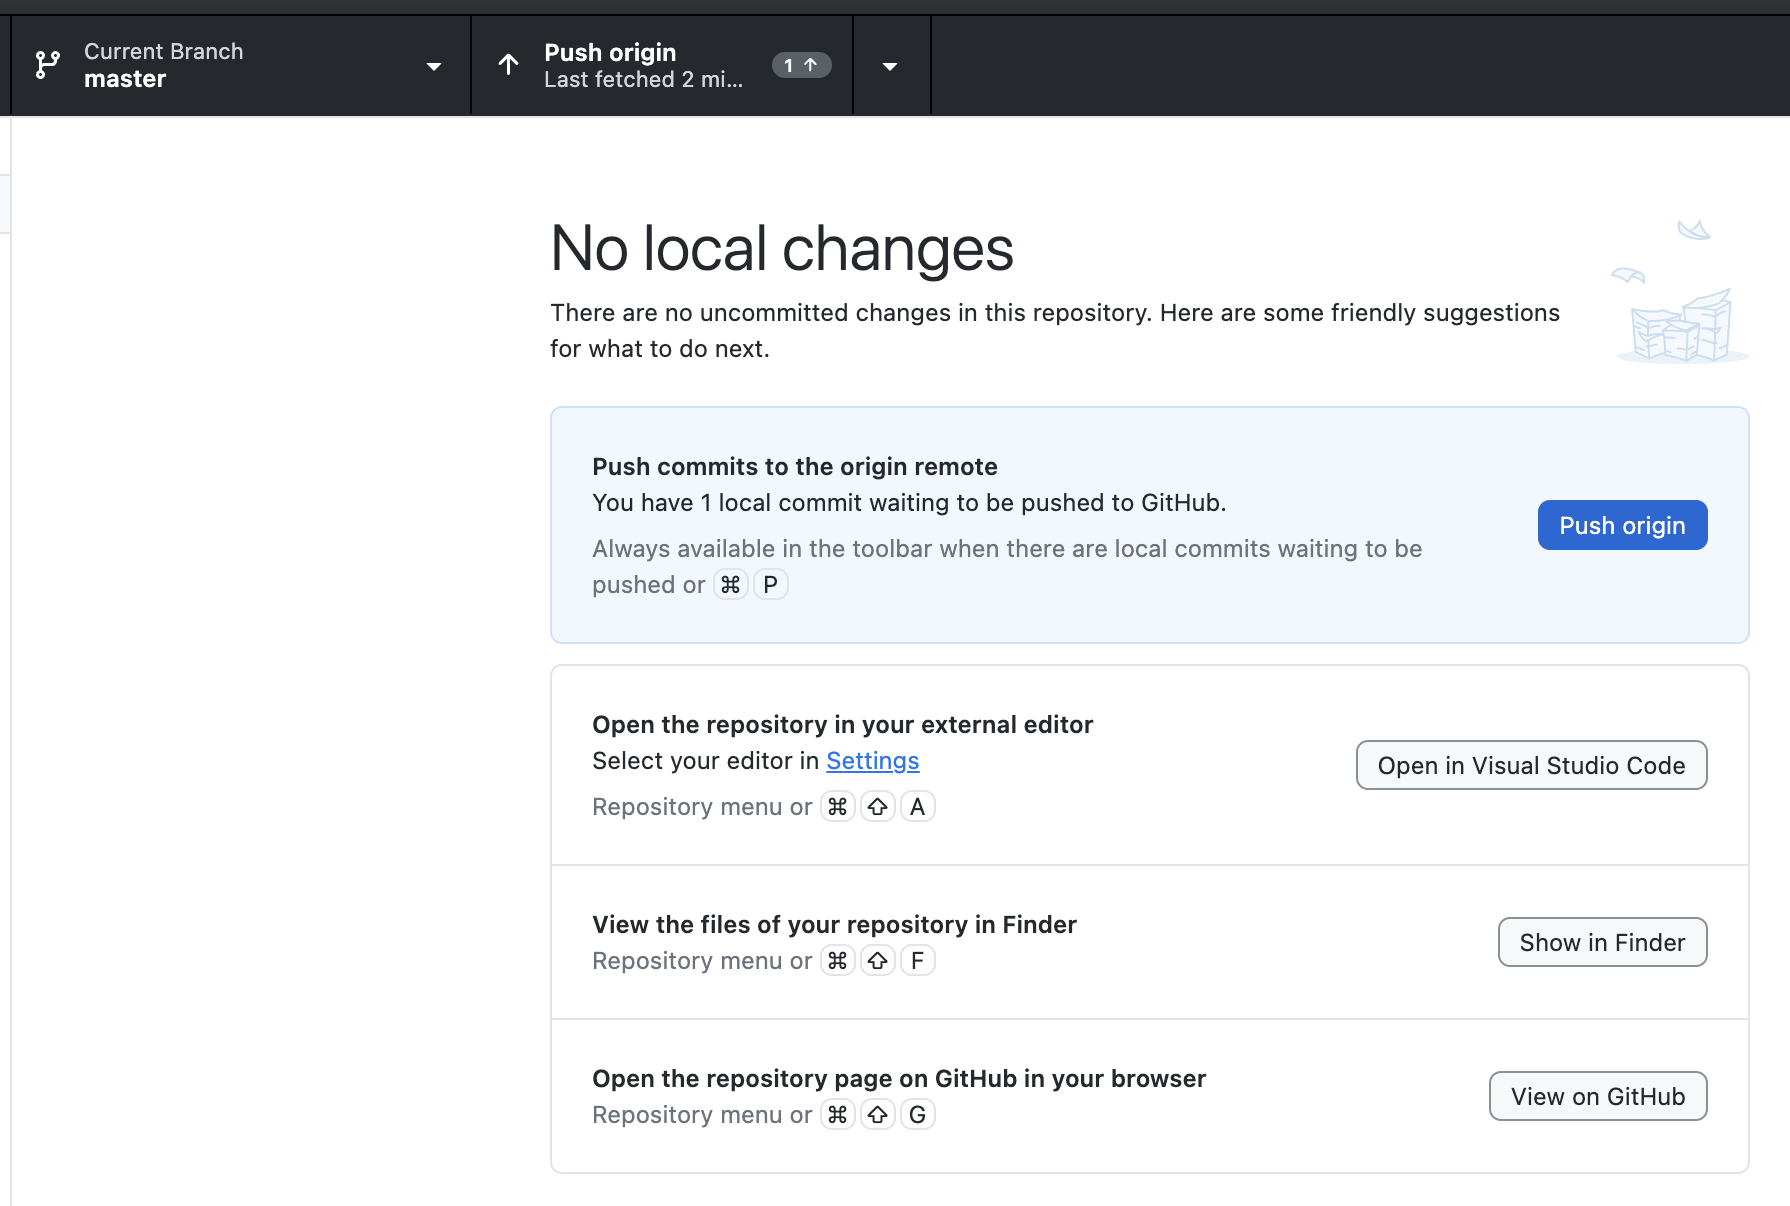
\includegraphics[width=1\linewidth]{Zrzut ekranu 2024-12-20 o 14.30.47.png}
    \caption{App window after committing all changes - an option to push stuff to the remote.}
    \label{fig:ghd-push}
\end{figure}

\section[Cloning a repo]{Cloning an existing online repo to your computer}\label{sec:cloning}
Although you can do it via \textit{Rstudio} or \textit{VSCode} - I recommend proceeding with \textit{GitHub Desktop}.

\subsection{GitHub Desktop}

In the app, navigate to the repository name and there, click \textbf{Add}, and then \textbf{Clone Repository}. In a window (fig.~\ref{fig:ghd-clone}) you will be asked to select an existing repository (since you're logged in - the app will provide you with a searchable list of all repositories you own or collaborate on). Pick the one you wish to clone, select the directory to host it locally and press \textbf{clone}. The content of your online repo will be transferred to your HDD - from now on you can access it via \textit{VSCode}, \textit{RStudio} or \textit{GitHub Desktop}, add things to it, commit and push/pull.

\begin{marginfigure}
    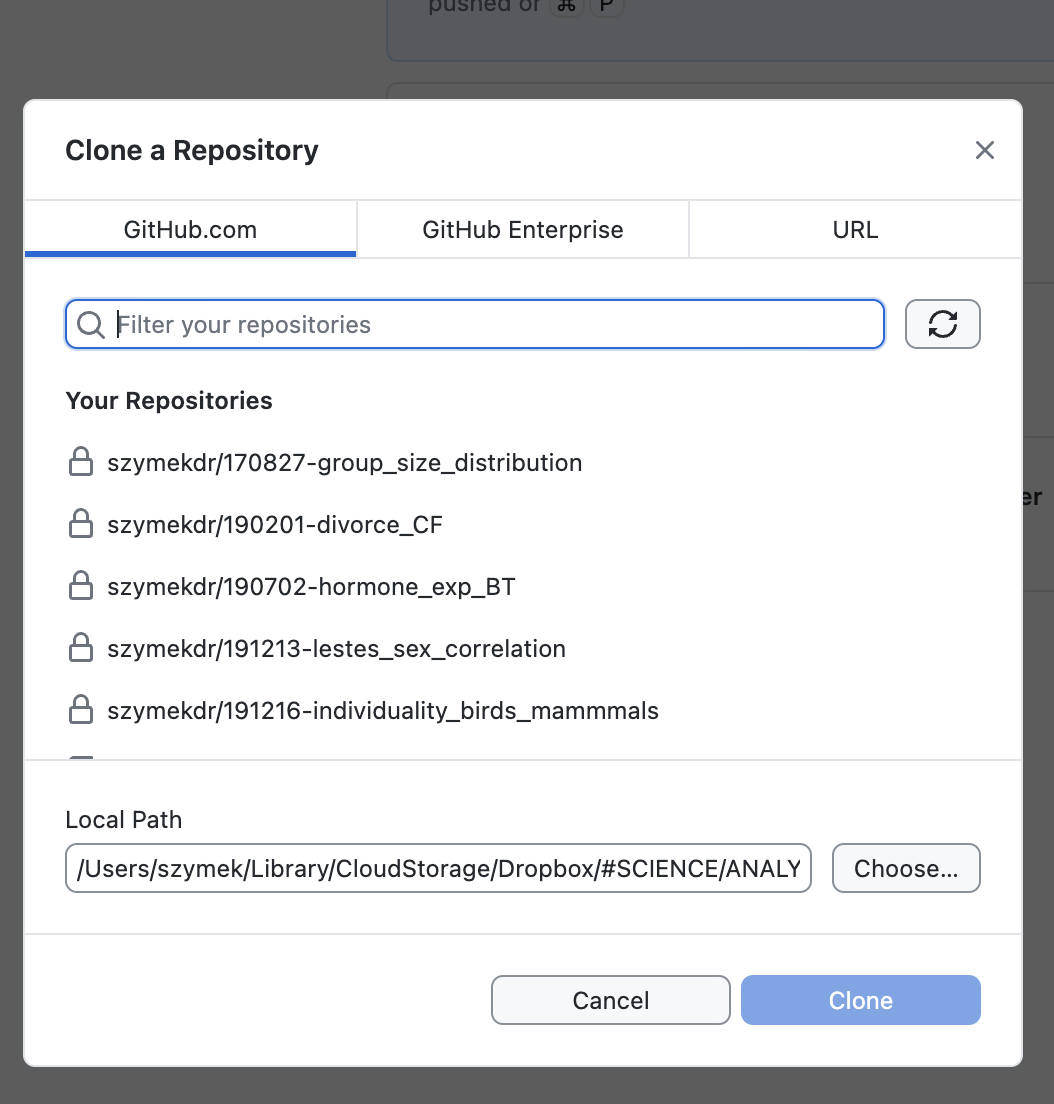
\includegraphics[width=1\linewidth]{Zrzut ekranu 2024-12-23 o 09.48.06.png}
    \caption{Repo cloning window in the desktop app}
    \label{fig:ghd-clone}
    \setfloatalignment{t}
\end{marginfigure}

If the repo you are cloning is your private fork of someone else's repository - the changes ou commit and push will of course update your instance of the repository, not the one from which it was forked. However, after pushing something to such a repo - you can navigate there online; the online system will alert you that your repo is \textit{ahead} of the original one by one or more commits (it may also be \textit{behind} - in which case you can be given an option to sync your fork with its parent). If you're indeed ahead of the parent one - you can send your changes as a pull request to the parent one, where its admins can review it and integrate into the repo's content.

\section{Our case: uploading data to the repository}

You are most likely a contributor to the Nestbox Experiment repository. This gives you several options to interact with it, and in particular - to deposit your data and other files into it.

\begin{enumerate}
    \item \textit{You have cloned the repo to your HDD}. In such case, before you proceed with any update, pull from the remote repository to make sure your local copy is in sync with the online one. Then place your fails in a selected location within the repository - e.g., in you study site's folder, or wherever was agreed among the contributors. Having done that, you should see the new/changed files as uncommitted changes in the Git panel of your app (or in \textit{GitHub Desktop}). Just commit the changes and push them up to the remote repository. All done!

    \item \textit{You don't have a local copy of the online repository.} If so, you can either follow the instructions in the section above to first clone everything to your HDD - or do everything online. In the latter case: just navigate to the repository's main page on \texttt{github.com}, go to the desired folder and pick \textbf{Upload files} (fig.~\ref{fig:upload}). Remember to avoid uploading files exceeding hundreds of megabytes.

    \begin{marginfigure}
        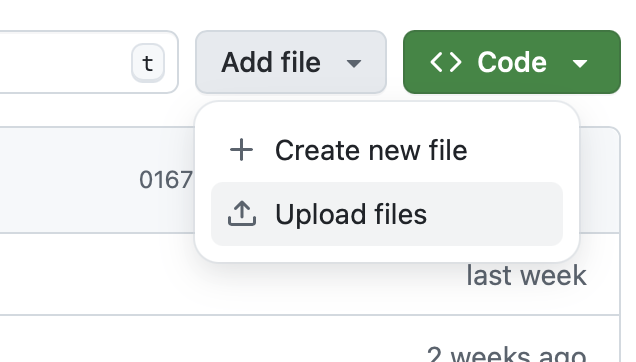
\includegraphics[width=1\linewidth]{Zrzut ekranu 2024-12-23 o 10.05.01.png}
        \caption{Uploading files online}
        \label{fig:upload}
        \setfloatalignment{t}
    \end{marginfigure}
\end{enumerate}

\section{Issues}

The online \textit{GitHub} service provides a number of tools that make collaboration easier. One of them is the system of \textit{Issues}. You can access them in your repo via the top menu bar (fig.~\ref{fig:issues}).

\begin{figure}
    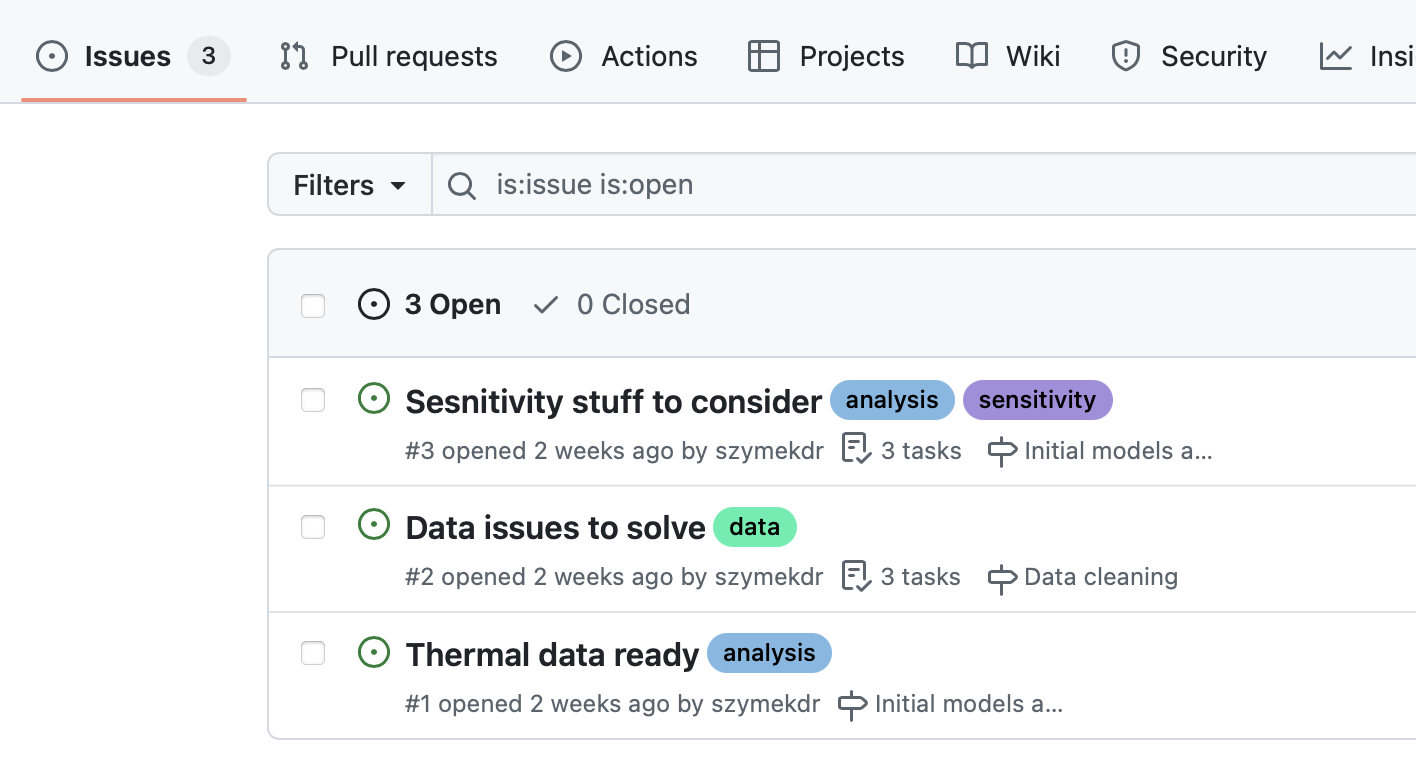
\includegraphics[width=1\linewidth]{Zrzut ekranu 2024-12-23 o 10.07.30.png}
    \caption{GitHub Issues}
    \label{fig:issues}
\end{figure}

The \textit{Issues} webpage is in fact a simple chat and discussion forum. You can create action topics there, you can even ping relevant contributors within each issue. It is a good practice to use this system to organise work, provide updates and communicate your progress on a task (and - of course - to close an issue once solved).

\end{document}
